\section{Описание}


Для анализа работы программы будем использовать утилиты valgrind, gprof и perf.
\begin{enumerate}
    \item \textbf{Valgrind} \newline
    Valgrind предназначен для отладки использования памяти, обнаружения утечек памяти, а также профилирования. Valgrind является по сути виртуальной машиной,
    использующей методы JIT-компиляции, среди которых – динамическая перекомпиляция. Valgrind транслитует программу во временную, более простую форму, называемую промежуточным представлением и работает с этим представлением.
    \item \textbf{Gprof} \newline
    Gprof – инструмент для анализа производительности UNIX приложений . Gprof вносит в программу дополнительный код на этапе компиляции, для извлечения необходимой информации.
    \item \textbf{Gcov} \newline
    Gcov — свободно распространяемая утилита для исследования покрытия кода. Gcov генерирует точное количество исполнений для каждого оператора в программе и позволяет добавить аннотации к исходному коду. Gcov поставляется как стандартная утилита в составе пакета GCC.
\end{enumerate}

\pagebreak

\section{Используемые средства}
\begin{enumerate}
    \item \textbf{Valgrind} \newline
    Утечки памяти одни из самых трудных для обнаружения ошибок, потому что они не вызывают никаких внешних проблем, до тех пор, пока у вас не закончится память и вам не удастся вызвать malloc. В самом деле, при работе с языками C или C++, которые не имеют сборки мусора, почти половину времени вы можете потратить на правильное освобождение памяти. И даже одна ошибка может дорого обойтись, если ваша программа работает достаточно долго и следует этой ветви кода
    \begin{alltt}
    root@Lunidep:~/DA/da_lab3/valgrind# g++ -Wall -Wextra -g da_lab2.cpp -o test_valgrind
    root@Lunidep:~/DA/da_lab3/valgrind# valgrind ./test_valgrind < tmp
    ==1572== Memcheck, a memory error detector
    ==1572== Copyright (C) 2002-2017, and GNU GPL'd, by Julian Seward et al.
    ==1572== Using Valgrind-3.15.0 and LibVEX; rerun with -h for copyright info
    ==1572== Command: ./test_valgrind 
    ==1572== 
    OK
    Exist
    OK
    OK: 18446744073709551615
    OK: 1
    OK
    NoSuchWord
    ==1572== 
    ==1572== HEAP SUMMARY:
    ==1572==     in use at exit: 122,880 bytes in 6 blocks
    ==1572==   total heap usage: 14 allocs, 8 frees, 196,997 bytes allocated
    ==1572== 
    ==1572== LEAK SUMMARY:
    ==1572==    definitely lost: 0 bytes in 0 blocks
    ==1572==    indirectly lost: 0 bytes in 0 blocks
    ==1572==      possibly lost: 0 bytes in 0 blocks
    ==1572==    still reachable: 122,880 bytes in 6 blocks
    ==1572==         suppressed: 0 bytes in 0 blocks
    ==1572== Rerun with --leak-check=full to see details of leaked memory
    ==1572== 
    ==1572== For lists of detected and suppressed errors, rerun with: -s
    ==1572== ERROR SUMMARY: 0 errors from 0 contexts (suppressed: 0 from 0)
    \end{alltt}
    Из полученных результатов можно сделать вывод, что явных утечек нет, но достижима утечка 122,880 байт.\newline
    Попробуем получить больше информации с помощью ключа –leak-check-full. Вследствие использования этого ключа можно установить, что причиной возможных утечек являются методы sync_with_stdio.\newline


    \item \textbf{Gprof} \newline
    Проверим время выполнения нашей программы с помощью Gprof. Для этого надо скомпилировать программу с флагом -pg(добавим этот флаг в CMakeLists.txt).\newline
    
    \begin{alltt}
    \footnotesize{
    root@Lunidep:~/DA/da_lab3/gprof# g++ -Wall -Wextra -pg benchmark.cpp -o test_gprof
    root@Lunidep:~/DA/da_lab3/gprof# ./test_gprof > /dev/null
    root@Lunidep:~/DA/da_lab3/gprof# ls
    benchmark.cpp  gmon.out  test_gprof  tmp
    root@Lunidep:~/DA/da_lab3/gprof# gprof test_gprof gmon.out > profile-data.txt
    Flat profile:
    
    Each sample counts as 0.01 seconds.
      %   cumulative   self              self     total           
     time   seconds   seconds    calls  ms/call  ms/call  name    
      9.93      0.25     0.25 77585158     0.00     0.00  void std::__cxx11::basic_string<char, std::char_traits<char>, std::allocator<char> >::_M_construct<char*>(char*, char*, std::forward_iterator_tag)
      8.34      0.46     0.21  2222008     0.00     0.00  std::_Rb_tree<std::__cxx11::basic_string<char, std::char_traits<char>, std::allocator<char> >, std::pair<std::__cxx11::basic_string<char, std::char_traits<char>, std::allocator<char> > const, unsigned long long>, std::_Select1st<std::pair<std::__cxx11::basic_string<char, std::char_traits<char>, std::allocator<char> > const, unsigned long long> >, std::less<std::__cxx11::basic_string<char, std::char_traits<char>, std::allocator<char> > >, std::allocator<std::pair<std::__cxx11::basic_string<char, std::char_traits<char>, std::allocator<char> > const, unsigned long long> > >::_M_get_insert_unique_pos(std::__cxx11::basic_string<char, std::char_traits<char>, std::allocator<char> > const&)
      6.75      0.63     0.17 277633680     0.00     0.00  TAvl<std::__cxx11::basic_string<char, std::char_traits<char>, std::allocator<char> >, unsigned long long>::Height(TAvl<std::__cxx11::basic_string<char, std::char_traits<char>, std::allocator<char> >, unsigned long long>::TAvlNode const*)
      6.75      0.80     0.17  2222008     0.00     0.00  TAvl<std::__cxx11::basic_string<char, std::char_traits<char>, std::allocator<char> >, unsigned long long>::Insert(TAvl<std::__cxx11::basic_string<char, std::char_traits<char>, std::allocator<char> >, unsigned long long>::TAvlNode*, std::__cxx11::basic_string<char, std::char_traits<char>, std::allocator<char> >, unsigned long long)
      5.96      0.95     0.15  8888032     0.00     0.00  std::__cxx11::basic_string<char, std::char_traits<char>, std::allocator<char> > __gnu_cxx::__to_xstring<std::__cxx11::basic_string<char, std::char_traits<char>, std::allocator<char> >, char>(int (*)(char*, unsigned long, char const*, __va_list_tag*), unsigned long, char const*, ...)
      4.77      1.07     0.12 71099550     0.00     0.00  TAvl<std::__cxx11::basic_string<char, std::char_traits<char>, std::allocator<char> >, unsigned long long>::Reheight(TAvl<std::__cxx11::basic_string<char, std::char_traits<char>, std::allocator<char> >, unsigned long long>::TAvlNode*)
      4.37      1.18     0.11 67717290     0.00     0.00  TAvl<std::__cxx11::basic_string<char, std::char_traits<char>, std::allocator<char> >, unsigned long long>::Balance(TAvl<std::__cxx11::basic_string<char, std::char_traits<char>, std::allocator<char> >, unsigned long long>::TAvlNode const*)
      3.57      1.27     0.09 66215747     0.00     0.00  TAvl<std::__cxx11::basic_string<char, std::char_traits<char>, std::allocator<char> >, unsigned long long>::Rebalance(TAvl<std::__cxx11::basic_string<char, std::char_traits<char>, std::allocator<char> >, unsigned long long>::TAvlNode*)
      2.98      1.35     0.08 77585158     0.00     0.00  std::iterator_traits<char*>::difference_type std::distance<char*>(char*, char*)
      2.78      1.42     0.07 118732749     0.00     0.00  std::less<std::__cxx11::basic_string<char, std::char_traits<char>, std::allocator<char> > >::operator()(std::__cxx11::basic_string<char, std::char_traits<char>, std::allocator<char> > const&, std::__cxx11::basic_string<char, std::char_traits<char>, std::allocator<char> > const&) const
      2.78      1.49     0.07 118732749     0.00     0.00  std::_Rb_tree<std::__cxx11::basic_string<char, std::char_traits<char>, std::allocator<char> >, std::pair<std::__cxx11::basic_string<char, std::char_traits<char>, std::allocator<char> > const, unsigned long long>, std::_Select1st<std::pair<std::__cxx11::basic_string<char, std::char_traits<char>, std::allocator<char> > const, unsigned long long> >, std::less<std::__cxx11::basic_string<char, std::char_traits<char>, std::allocator<char> > >, std::allocator<std::pair<std::__cxx11::basic_string<char, std::char_traits<char>, std::allocator<char> > const, unsigned long long> > >::_S_key(std::_Rb_tree_node<std::pair<std::__cxx11::basic_string<char, std::char_traits<char>, std::allocator<char> > const, unsigned long long> > const*)
      2.78      1.56     0.07 71099550     0.00     0.00  unsigned long long const& std::max<unsigned long long>(unsigned long long const&, unsigned long long const&)
      2.38      1.62     0.06 65195182     0.00     0.00  std::_Rb_tree<std::__cxx11::basic_string<char, std::char_traits<char>, std::allocator<char> >, std::pair<std::__cxx11::basic_string<char, std::char_traits<char>, std::allocator<char> > const, unsigned long long>, std::_Select1st<std::pair<std::__cxx11::basic_string<char, std::char_traits<char>, std::allocator<char> > const, unsigned long long> >, std::less<std::__cxx11::basic_string<char, std::char_traits<char>, std::allocator<char> > >, std::allocator<std::pair<std::__cxx11::basic_string<char, std::char_traits<char>, std::allocator<char> > const, unsigned long long> > >::_S_right(std::_Rb_tree_node_base*)
      2.38      1.68     0.06 203662318     0.00     0.00  bool std::operator< <char, std::char_traits<char>, std::allocator<char> >(std::__cxx11::basic_string<char, std::char_traits<char>, std::allocator<char> > const&, std::__cxx11::basic_string<char, std::char_traits<char>, std::allocator<char> > const&)
      2.38      1.74     0.06  1111004     0.00     0.00  TAvl<std::__cxx11::basic_string<char, std::char_traits<char>, std::allocator<char> >, unsigned long long>::Search(TAvl<std::__cxx11::basic_string<char, std::char_traits<char>, std::allocator<char> >, unsigned long long>::TAvlNode*, std::__cxx11::basic_string<char, std::char_traits<char>, std::allocator<char> >)
      1.99      1.79     0.05  2222008     0.00     0.00  TAvl<std::__cxx11::basic_string<char, std::char_traits<char>, std::allocator<char> >, unsigned long long>::Add(std::__cxx11::basic_string<char, std::char_traits<char>, std::allocator<char> >, unsigned long long)
      1.99      1.84     0.05  1111004     0.00     0.00  std::_Rb_tree<std::__cxx11::basic_string<char, std::char_traits<char>, std::allocator<char> >, std::pair<std::__cxx11::basic_string<char, std::char_traits<char>, std::allocator<char> > const, unsigned long long>, std::_Select1st<std::pair<std::__cxx11::basic_string<char, std::char_traits<char>, std::allocator<char> > const, unsigned long long> >, std::less<std::__cxx11::basic_string<char, std::char_traits<char>, std::allocator<char> > >, std::allocator<std::pair<std::__cxx11::basic_string<char, std::char_traits<char>, std::allocator<char> > const, unsigned long long> > >::equal_range(std::__cxx11::basic_string<char, std::char_traits<char>, std::allocator<char> > const&)
      1.99      1.89     0.05 49213654     0.00     0.00  bool std::operator><char, std::char_traits<char>, std::allocator<char> >(std::__cxx11::basic_string<char, std::char_traits<char>, std::allocator<char> > const&, std::__cxx11::basic_string<char, std::char_traits<char>, std::allocator<char> > const&)
      1.59      1.93     0.04 118732749     0.00     0.00  __gnu_cxx::__aligned_membuf<std::pair<std::__cxx11::basic_string<char, std::char_traits<char>, std::allocator<char> > const, unsigned long long> >::_M_ptr() const
      1.59      1.97     0.04  2111005     0.00     0.00  std::_Rb_tree_iterator<std::pair<std::__cxx11::basic_string<char, std::char_traits<char>, std::allocator<char> > const, unsigned long long> > std::_Rb_tree<std::__cxx11::basic_string<char, std::char_traits<char>, std::allocator<char> >, std::pair<std::__cxx11::basic_string<char, std::char_traits<char>, std::allocator<char> > const, unsigned long long>, std::_Select1st<std::pair<std::__cxx11::basic_string<char, std::char_traits<char>, std::allocator<char> > const, unsigned long long> >, std::less<std::__cxx11::basic_string<char, std::char_traits<char>, std::allocator<char> > >, std::allocator<std::pair<std::__cxx11::basic_string<char, std::char_traits<char>, std::allocator<char> > const, unsigned long long> > >::_M_insert_<std::pair<std::__cxx11::basic_string<char, std::char_traits<char>, std::allocator<char> > const, unsigned long long>, std::_Rb_tree<std::__cxx11::basic_string<char, std::char_traits<char>, std::allocator<char> >, std::pair<std::__cxx11::basic_string<char, std::char_traits<char>, std::allocator<char> > const, unsigned long long>, std::_Select1st<std::pair<std::__cxx11::basic_string<char, std::char_traits<char>, std::allocator<char> > const, unsigned long long> >, std::less<std::__cxx11::basic_string<char, std::char_traits<char>, std::allocator<char> > >, std::allocator<std::pair<std::__cxx11::basic_string<char, std::char_traits<char>, std::allocator<char> > const, unsigned long long> > >::_Alloc_node>(std::_Rb_tree_node_base*, std::_Rb_tree_node_base*, std::pair<std::__cxx11::basic_string<char, std::char_traits<char>, std::allocator<char> > const, unsigned long long>&&, std::_Rb_tree<std::__cxx11::basic_string<char, std::char_traits<char>, std::allocator<char> >, std::pair<std::__cxx11::basic_string<char, std::char_traits<char>, std::allocator<char> > const, unsigned long long>, std::_Select1st<std::pair<std::__cxx11::basic_string<char, std::char_traits<char>, std::allocator<char> > const, unsigned long long> >, std::less<std::__cxx11::basic_string<char, std::char_traits<char>, std::allocator<char> > >, std::allocator<std::pair<std::__cxx11::basic_string<char, std::char_traits<char>, std::allocator<char> > const, unsigned long long> > >::_Alloc_node&)
      1.39      2.00     0.04 77585158     0.00     0.00  bool __gnu_cxx::__is_null_pointer<char>(char*)
      1.19      2.03     0.03  8888032     0.00     0.00  std::__cxx11::basic_string<char, std::char_traits<char>, std::allocator<char> >::basic_string<char*, void>(char*, char*, std::allocator<char> const&)
      1.19      2.06     0.03  2222008     0.00     0.00  std::_Rb_tree<std::__cxx11::basic_string<char, std::char_traits<char>, std::allocator<char> >, std::pair<std::__cxx11::basic_string<char, std::char_traits<char>, std::allocator<char> > const, unsigned long long>, std::_Select1st<std::pair<std::__cxx11::basic_string<char, std::char_traits<char>, std::allocator<char> > const, unsigned long long> >, std::less<std::__cxx11::basic_string<char, std::char_traits<char>, std::allocator<char> > >, std::allocator<std::pair<std::__cxx11::basic_string<char, std::char_traits<char>, std::allocator<char> > const, unsigned long long> > >::_M_lower_bound(std::_Rb_tree_node<std::pair<std::__cxx11::basic_string<char, std::char_traits<char>, std::allocator<char> > const, unsigned long long> >*, std::_Rb_tree_node_base*, std::__cxx11::basic_string<char, std::char_traits<char>, std::allocator<char> > const&)
      1.19      2.09     0.03  2111005     0.00     0.00  void __gnu_cxx::new_allocator<std::_Rb_tree_node<std::pair<std::__cxx11::basic_string<char, std::char_traits<char>, std::allocator<char> > const, unsigned long long> > >::construct<std::pair<std::__cxx11::basic_string<char, std::char_traits<char>, std::allocator<char> > const, unsigned long long>, std::pair<std::__cxx11::basic_string<char, std::char_traits<char>, std::allocator<char> > const, unsigned long long> >(std::pair<std::__cxx11::basic_string<char, std::char_traits<char>, std::allocator<char> > const, unsigned long long>*, std::pair<std::__cxx11::basic_string<char, std::char_traits<char>, std::allocator<char> > const, unsigned long long>&&)
      1.19      2.12     0.03  1111004     0.00     0.00  TAvl<std::__cxx11::basic_string<char, std::char_traits<char>, std::allocator<char> >, unsigned long long>::Remove(TAvl<std::__cxx11::basic_string<char, std::char_traits<char>, std::allocator<char> >, unsigned long long>::TAvlNode*, std::__cxx11::basic_string<char, std::char_traits<char>, std::allocator<char> >)
      0.99      2.15     0.03 118732749     0.00     0.00  __gnu_cxx::__aligned_membuf<std::pair<std::__cxx11::basic_string<char, std::char_traits<char>, std::allocator<char> > const, unsigned long long> >::_M_addr() const
      0.99      2.17     0.03 41281958     0.00     0.00  std::_Rb_tree<std::__cxx11::basic_string<char, std::char_traits<char>, std::allocator<char> >, std::pair<std::__cxx11::basic_string<char, std::char_traits<char>, std::allocator<char> > const, unsigned long long>, std::_Select1st<std::pair<std::__cxx11::basic_string<char, std::char_traits<char>, std::allocator<char> > const, unsigned long long> >, std::less<std::__cxx11::basic_string<char, std::char_traits<char>, std::allocator<char> > >, std::allocator<std::pair<std::__cxx11::basic_string<char, std::char_traits<char>, std::allocator<char> > const, unsigned long long> > >::_S_left(std::_Rb_tree_node_base*)
      0.79      2.19     0.02 118732749     0.00     0.00  std::_Select1st<std::pair<std::__cxx11::basic_string<char, std::char_traits<char>, std::allocator<char> > const, unsigned long long> >::operator()(std::pair<std::__cxx11::basic_string<char, std::char_traits<char>, std::allocator<char> > const, unsigned long long> const&) const
      0.79      2.21     0.02 77585158     0.00     0.00  std::iterator_traits<char*>::difference_type std::__distance<char*>(char*, char*, std::random_access_iterator_tag)
      0.79      2.23     0.02 10405436     0.00     0.00  std::_Rb_tree_iterator<std::pair<std::__cxx11::basic_string<char, std::char_traits<char>, std::allocator<char> > const, unsigned long long> >::_Rb_tree_iterator(std::_Rb_tree_node_base*)
      0.79      2.25     0.02  8888032     0.00     0.00  std::__cxx11::to_string(int)
      0.79      2.27     0.02  2222008     0.00     0.00  std::pair<std::_Rb_tree_iterator<std::pair<std::__cxx11::basic_string<char, std::char_traits<char>, std::allocator<char> > const, unsigned long long> >, bool> std::_Rb_tree<std::__cxx11::basic_string<char, std::char_traits<char>, std::allocator<char> >, std::pair<std::__cxx11::basic_string<char, std::char_traits<char>, std::allocator<char> > const, unsigned long long>, std::_Select1st<std::pair<std::__cxx11::basic_string<char, std::char_traits<char>, std::allocator<char> > const, unsigned long long> >, std::less<std::__cxx11::basic_string<char, std::char_traits<char>, std::allocator<char> > >, std::allocator<std::pair<std::__cxx11::basic_string<char, std::char_traits<char>, std::allocator<char> > const, unsigned long long> > >::_M_insert_unique<std::pair<std::__cxx11::basic_string<char, std::char_traits<char>, std::allocator<char> > const, unsigned long long> >(std::pair<std::__cxx11::basic_string<char, std::char_traits<char>, std::allocator<char> > const, unsigned long long>&&)
      0.79      2.29     0.02  2111005     0.00     0.00  __gnu_cxx::new_allocator<std::_Rb_tree_node<std::pair<std::__cxx11::basic_string<char, std::char_traits<char>, std::allocator<char> > const, unsigned long long> > >::deallocate(std::_Rb_tree_node<std::pair<std::__cxx11::basic_string<char, std::char_traits<char>, std::allocator<char> > const, unsigned long long> >*, unsigned long)
      0.79      2.31     0.02  2111005     0.00     0.00  std::_Rb_tree<std::__cxx11::basic_string<char, std::char_traits<char>, std::allocator<char> >, std::pair<std::__cxx11::basic_string<char, std::char_traits<char>, std::allocator<char> > const, unsigned long long>, std::_Select1st<std::pair<std::__cxx11::basic_string<char, std::char_traits<char>, std::allocator<char> > const, unsigned long long> >, std::less<std::__cxx11::basic_string<char, std::char_traits<char>, std::allocator<char> > >, std::allocator<std::pair<std::__cxx11::basic_string<char, std::char_traits<char>, std::allocator<char> > const, unsigned long long> > >::_M_put_node(std::_Rb_tree_node<std::pair<std::__cxx11::basic_string<char, std::char_traits<char>, std::allocator<char> > const, unsigned long long> >*)
      0.79      2.33     0.02  2111005     0.00     0.00  void std::_Rb_tree<std::__cxx11::basic_string<char, std::char_traits<char>, std::allocator<char> >, std::pair<std::__cxx11::basic_string<char, std::char_traits<char>, std::allocator<char> > const, unsigned long long>, std::_Select1st<std::pair<std::__cxx11::basic_string<char, std::char_traits<char>, std::allocator<char> > const, unsigned long long> >, std::less<std::__cxx11::basic_string<char, std::char_traits<char>, std::allocator<char> > >, std::allocator<std::pair<std::__cxx11::basic_string<char, std::char_traits<char>, std::allocator<char> > const, unsigned long long> > >::_M_construct_node<std::pair<std::__cxx11::basic_string<char, std::char_traits<char>, std::allocator<char> > const, unsigned long long> >(std::_Rb_tree_node<std::pair<std::__cxx11::basic_string<char, std::char_traits<char>, std::allocator<char> > const, unsigned long long> >*, std::pair<std::__cxx11::basic_string<char, std::char_traits<char>, std::allocator<char> > const, unsigned long long>&&)
      0.79      2.35     0.02   893897     0.00     0.00  TAvl<std::__cxx11::basic_string<char, std::char_traits<char>, std::allocator<char> >, unsigned long long>::RemoveMin(TAvl<std::__cxx11::basic_string<char, std::char_traits<char>, std::allocator<char> >, unsigned long long>::TAvlNode*, TAvl<std::__cxx11::basic_string<char, std::char_traits<char>, std::allocator<char> >, unsigned long long>::TAvlNode*)
      0.40      2.36     0.01 118732749     0.00     0.00  std::_Rb_tree_node<std::pair<std::__cxx11::basic_string<char, std::char_traits<char>, std::allocator<char> > const, unsigned long long> >::_M_valptr() const
      0.40      2.37     0.01 77585158     0.00     0.00  std::iterator_traits<char*>::iterator_category std::__iterator_category<char*>(char* const&)
      0.40      2.38     0.01  8888032     0.00     0.00  void std::__cxx11::basic_string<char, std::char_traits<char>, std::allocator<char> >::_M_construct<char*>(char*, char*)
      0.40      2.39     0.01  6666024     0.00     0.00  std::chrono::duration<long, std::ratio<1l, 1000000l> >::count() const
      0.40      2.40     0.01  6666024     0.00     0.00  std::enable_if<std::chrono::__is_duration<std::chrono::duration<long, std::ratio<1l, 1000000l> > >::value, std::chrono::duration<long, std::ratio<1l, 1000000l> > >::type std::chrono::duration_cast<std::chrono::duration<long, std::ratio<1l, 1000000l> >, long, std::ratio<1l, 1000000000l> >(std::chrono::duration<long, std::ratio<1l, 1000000000l> > const&)
      0.40      2.41     0.01  4444017     0.00     0.00  std::_Rb_tree<std::__cxx11::basic_string<char, std::char_traits<char>, std::allocator<char> >, std::pair<std::__cxx11::basic_string<char, std::char_traits<char>, std::allocator<char> > const, unsigned long long>, std::_Select1st<std::pair<std::__cxx11::basic_string<char, std::char_traits<char>, std::allocator<char> > const, unsigned long long> >, std::less<std::__cxx11::basic_string<char, std::char_traits<char>, std::allocator<char> > >, std::allocator<std::pair<std::__cxx11::basic_string<char, std::char_traits<char>, std::allocator<char> > const, unsigned long long> > >::_M_begin()
      0.40      2.42     0.01  2222008     0.00     0.00  std::_Rb_tree<std::__cxx11::basic_string<char, std::char_traits<char>, std::allocator<char> >, std::pair<std::__cxx11::basic_string<char, std::char_traits<char>, std::allocator<char> > const, unsigned long long>, std::_Select1st<std::pair<std::__cxx11::basic_string<char, std::char_traits<char>, std::allocator<char> > const, unsigned long long> >, std::less<std::__cxx11::basic_string<char, std::char_traits<char>, std::allocator<char> > >, std::allocator<std::pair<std::__cxx11::basic_string<char, std::char_traits<char>, std::allocator<char> > const, unsigned long long> > >::size() const
      0.40      2.43     0.01  2222008     0.00     0.00  std::pair<std::__cxx11::basic_string<char, std::char_traits<char>, std::allocator<char> > const, unsigned long long>::pair<std::__cxx11::basic_string<char, std::char_traits<char>, std::allocator<char> >, int&, true>(std::__cxx11::basic_string<char, std::char_traits<char>, std::allocator<char> >&&, int&)
      0.40      2.44     0.01  2111005     0.00     0.00  void __gnu_cxx::new_allocator<std::_Rb_tree_node<std::pair<std::__cxx11::basic_string<char, std::char_traits<char>, std::allocator<char> > const, unsigned long long> > >::destroy<std::pair<std::__cxx11::basic_string<char, std::char_traits<char>, std::allocator<char> > const, unsigned long long> >(std::pair<std::__cxx11::basic_string<char, std::char_traits<char>, std::allocator<char> > const, unsigned long long>*)
      0.40      2.45     0.01  2111005     0.00     0.00  std::allocator_traits<std::allocator<std::_Rb_tree_node<std::pair<std::__cxx11::basic_string<char, std::char_traits<char>, std::allocator<char> > const, unsigned long long> > > >::deallocate(std::allocator<std::_Rb_tree_node<std::pair<std::__cxx11::basic_string<char, std::char_traits<char>, std::allocator<char> > const, unsigned long long> > >&, std::_Rb_tree_node<std::pair<std::__cxx11::basic_string<char, std::char_traits<char>, std::allocator<char> > const, unsigned long long> >*, unsigned long)
      0.40      2.46     0.01  2111005     0.00     0.00  std::pair<std::__cxx11::basic_string<char, std::char_traits<char>, std::allocator<char> > const, unsigned long long>::pair(std::pair<std::__cxx11::basic_string<char, std::char_traits<char>, std::allocator<char> > const, unsigned long long>&&)
      0.40      2.47     0.01  2111005     0.00     0.00  std::pair<std::_Rb_tree_node_base*, std::_Rb_tree_node_base*>::pair<std::_Rb_tree_node<std::pair<std::__cxx11::basic_string<char, std::char_traits<char>, std::allocator<char> > const, unsigned long long> >*&, std::_Rb_tree_node_base*&, true>(std::_Rb_tree_node<std::pair<std::__cxx11::basic_string<char, std::char_traits<char>, std::allocator<char> > const, unsigned long long> >*&, std::_Rb_tree_node_base*&)
      0.40      2.48     0.01  1111004     0.00     0.00  std::_Rb_tree<std::__cxx11::basic_string<char, std::char_traits<char>, std::allocator<char> >, std::pair<std::__cxx11::basic_string<char, std::char_traits<char>, std::allocator<char> > const, unsigned long long>, std::_Select1st<std::pair<std::__cxx11::basic_string<char, std::char_traits<char>, std::allocator<char> > const, unsigned long long> >, std::less<std::__cxx11::basic_string<char, std::char_traits<char>, std::allocator<char> > >, std::allocator<std::pair<std::__cxx11::basic_string<char, std::char_traits<char>, std::allocator<char> > const, unsigned long long> > >::_M_erase_aux(std::_Rb_tree_const_iterator<std::pair<std::__cxx11::basic_string<char, std::char_traits<char>, std::allocator<char> > const, unsigned long long> >, std::_Rb_tree_const_iterator<std::pair<std::__cxx11::basic_string<char, std::char_traits<char>, std::allocator<char> > const, unsigned long long> >)
      0.40      2.49     0.01  1111004     0.00     0.00  std::_Rb_tree<std::__cxx11::basic_string<char, std::char_traits<char>, std::allocator<char> >, std::pair<std::__cxx11::basic_string<char, std::char_traits<char>, std::allocator<char> > const, unsigned long long>, std::_Select1st<std::pair<std::__cxx11::basic_string<char, std::char_traits<char>, std::allocator<char> > const, unsigned long long> >, std::less<std::__cxx11::basic_string<char, std::char_traits<char>, std::allocator<char> > >, std::allocator<std::pair<std::__cxx11::basic_string<char, std::char_traits<char>, std::allocator<char> > const, unsigned long long> > >::find(std::__cxx11::basic_string<char, std::char_traits<char>, std::allocator<char> > const&)
      0.40      2.50     0.01        1    10.01    10.01  TAvl<std::__cxx11::basic_string<char, std::char_traits<char>, std::allocator<char> >, unsigned long long>::TreeDelete(TAvl<std::__cxx11::basic_string<char, std::char_traits<char>, std::allocator<char> >, unsigned long long>::TAvlNode*)
      0.40      2.51     0.01                             main
      0.20      2.52     0.01  4222010     0.00     0.00  __gnu_cxx::__aligned_membuf<std::pair<std::__cxx11::basic_string<char, std::char_traits<char>, std::allocator<char> > const, unsigned long long> >::_M_addr()
      0.20      2.52     0.01        1     5.00     5.00  __gnu_cxx::new_allocator<std::_Rb_tree_node<std::pair<std::__cxx11::basic_string<char, std::char_traits<char>, std::allocator<char> > const, unsigned long long> > >::new_allocator()
      0.00      2.52     0.00 19998072     0.00     0.00  std::chrono::duration<long, std::ratio<1l, 1000000000l> >::count() const
      0.00      2.52     0.00 14777035     0.00     0.00  std::pair<std::__cxx11::basic_string<char, std::char_traits<char>, std::allocator<char> > const, unsigned long long>&& std::forward<std::pair<std::__cxx11::basic_string<char, std::char_traits<char>, std::allocator<char> > const, unsigned long long> >(std::remove_reference<std::pair<std::__cxx11::basic_string<char, std::char_traits<char>, std::allocator<char> > const, unsigned long long> >::type&)
      0.00      2.52     0.00 13332048     0.00     0.00  std::chrono::time_point<std::chrono::_V2::system_clock, std::chrono::duration<long, std::ratio<1l, 1000000000l> > >::time_since_epoch() const
      0.00      2.52     0.00  8888032     0.00     0.00  void std::__cxx11::basic_string<char, std::char_traits<char>, std::allocator<char> >::_M_construct_aux<char*>(char*, char*, std::__false_type)
      0.00      2.52     0.00  8444020     0.00     0.00  std::_Rb_tree<std::__cxx11::basic_string<char, std::char_traits<char>, std::allocator<char> >, std::pair<std::__cxx11::basic_string<char, std::char_traits<char>, std::allocator<char> > const, unsigned long long>, std::_Select1st<std::pair<std::__cxx11::basic_string<char, std::char_traits<char>, std::allocator<char> > const, unsigned long long> >, std::less<std::__cxx11::basic_string<char, std::char_traits<char>, std::allocator<char> > >, std::allocator<std::pair<std::__cxx11::basic_string<char, std::char_traits<char>, std::allocator<char> > const, unsigned long long> > >::_M_get_Node_allocator()
      0.00      2.52     0.00  6666024     0.00     0.00  std::chrono::duration<long, std::ratio<1l, 1000000l> > std::chrono::__duration_cast_impl<std::chrono::duration<long, std::ratio<1l, 1000000l> >, std::ratio<1l, 1000l>, long, true, false>::__cast<long, std::ratio<1l, 1000000000l> >(std::chrono::duration<long, std::ratio<1l, 1000000000l> > const&)
      0.00      2.52     0.00  6666024     0.00     0.00  std::chrono::duration<long, std::ratio<1l, 1000000000l> >::duration<long, void>(long const&)
      0.00      2.52     0.00  6666024     0.00     0.00  std::chrono::duration<long, std::ratio<1l, 1000000l> >::duration<long, void>(long const&)
      0.00      2.52     0.00  6666024     0.00     0.00  std::common_type<std::chrono::duration<long, std::ratio<1l, 1000000000l> >, std::chrono::duration<long, std::ratio<1l, 1000000000l> > >::type std::chrono::operator-<std::chrono::_V2::system_clock, std::chrono::duration<long, std::ratio<1l, 1000000000l> >, std::chrono::duration<long, std::ratio<1l, 1000000000l> > >(std::chrono::time_point<std::chrono::_V2::system_clock, std::chrono::duration<long, std::ratio<1l, 1000000000l> > > const&, std::chrono::time_point<std::chrono::_V2::system_clock, std::chrono::duration<long, std::ratio<1l, 1000000000l> > > const&)
      0.00      2.52     0.00  6666024     0.00     0.00  std::common_type<std::chrono::duration<long, std::ratio<1l, 1000000000l> >, std::chrono::duration<long, std::ratio<1l, 1000000000l> > >::type std::chrono::operator-<long, std::ratio<1l, 1000000000l>, long, std::ratio<1l, 1000000000l> >(std::chrono::duration<long, std::ratio<1l, 1000000000l> > const&, std::chrono::duration<long, std::ratio<1l, 1000000000l> > const&)
      0.00      2.52     0.00  6555021     0.00     0.00  std::_Rb_tree<std::__cxx11::basic_string<char, std::char_traits<char>, std::allocator<char> >, std::pair<std::__cxx11::basic_string<char, std::char_traits<char>, std::allocator<char> > const, unsigned long long>, std::_Select1st<std::pair<std::__cxx11::basic_string<char, std::char_traits<char>, std::allocator<char> > const, unsigned long long> >, std::less<std::__cxx11::basic_string<char, std::char_traits<char>, std::allocator<char> > >, std::allocator<std::pair<std::__cxx11::basic_string<char, std::char_traits<char>, std::allocator<char> > const, unsigned long long> > >::_M_end()
      0.00      2.52     0.00  5444011     0.00     0.00  std::_Rb_tree<std::__cxx11::basic_string<char, std::char_traits<char>, std::allocator<char> >, std::pair<std::__cxx11::basic_string<char, std::char_traits<char>, std::allocator<char> > const, unsigned long long>, std::_Select1st<std::pair<std::__cxx11::basic_string<char, std::char_traits<char>, std::allocator<char> > const, unsigned long long> >, std::less<std::__cxx11::basic_string<char, std::char_traits<char>, std::allocator<char> > >, std::allocator<std::pair<std::__cxx11::basic_string<char, std::char_traits<char>, std::allocator<char> > const, unsigned long long> > >::_S_key(std::_Rb_tree_node_base const*)
      0.00      2.52     0.00  5337913     0.00     0.00  std::remove_reference<std::__cxx11::basic_string<char, std::char_traits<char>, std::allocator<char> >&>::type&& std::move<std::__cxx11::basic_string<char, std::char_traits<char>, std::allocator<char> >&>(std::__cxx11::basic_string<char, std::char_traits<char>, std::allocator<char> >&)
      0.00      2.52     0.00  4444016     0.00     0.00  std::_Rb_tree_iterator<std::pair<std::__cxx11::basic_string<char, std::char_traits<char>, std::allocator<char> > const, unsigned long long> >&& std::forward<std::_Rb_tree_iterator<std::pair<std::__cxx11::basic_string<char, std::char_traits<char>, std::allocator<char> > const, unsigned long long> > >(std::remove_reference<std::_Rb_tree_iterator<std::pair<std::__cxx11::basic_string<char, std::char_traits<char>, std::allocator<char> > const, unsigned long long> > >::type&)
      0.00      2.52     0.00  4333013     0.00     0.00  std::pair<std::__cxx11::basic_string<char, std::char_traits<char>, std::allocator<char> > const, unsigned long long>::~pair()
      0.00      2.52     0.00  4333012     0.00     0.00  std::_Select1st<std::pair<std::__cxx11::basic_string<char, std::char_traits<char>, std::allocator<char> > const, unsigned long long> >::operator()(std::pair<std::__cxx11::basic_string<char, std::char_traits<char>, std::allocator<char> > const, unsigned long long>&) const
      0.00      2.52     0.00  4222010     0.00     0.00  __gnu_cxx::__aligned_membuf<std::pair<std::__cxx11::basic_string<char, std::char_traits<char>, std::allocator<char> > const, unsigned long long> >::_M_ptr()
      0.00      2.52     0.00  4222010     0.00     0.00  std::_Rb_tree_node<std::pair<std::__cxx11::basic_string<char, std::char_traits<char>, std::allocator<char> > const, unsigned long long> >::_M_valptr()
      0.00      2.52     0.00  4222010     0.00     0.00  operator new(unsigned long, void*)
      0.00      2.52     0.00  3333016     0.00     0.00  std::_Rb_tree_const_iterator<std::pair<std::__cxx11::basic_string<char, std::char_traits<char>, std::allocator<char> > const, unsigned long long> >::_Rb_tree_const_iterator(std::_Rb_tree_iterator<std::pair<std::__cxx11::basic_string<char, std::char_traits<char>, std::allocator<char> > const, unsigned long long> > const&)
      0.00      2.52     0.00  2222008     0.00     0.00  std::map<std::__cxx11::basic_string<char, std::char_traits<char>, std::allocator<char> >, unsigned long long, std::less<std::__cxx11::basic_string<char, std::char_traits<char>, std::allocator<char> > >, std::allocator<std::pair<std::__cxx11::basic_string<char, std::char_traits<char>, std::allocator<char> > const, unsigned long long> > >::insert(std::pair<std::__cxx11::basic_string<char, std::char_traits<char>, std::allocator<char> > const, unsigned long long>&&)
      0.00      2.52     0.00  2222008     0.00     0.00  std::pair<std::_Rb_tree_iterator<std::pair<std::__cxx11::basic_string<char, std::char_traits<char>, std::allocator<char> > const, unsigned long long> >, bool>::pair<std::_Rb_tree_iterator<std::pair<std::__cxx11::basic_string<char, std::char_traits<char>, std::allocator<char> > const, unsigned long long> >, bool, true>(std::_Rb_tree_iterator<std::pair<std::__cxx11::basic_string<char, std::char_traits<char>, std::allocator<char> > const, unsigned long long> >&&, bool&&)
      0.00      2.52     0.00  2222008     0.00     0.00  std::remove_reference<std::pair<std::__cxx11::basic_string<char, std::char_traits<char>, std::allocator<char> > const, unsigned long long>&>::type&& std::move<std::pair<std::__cxx11::basic_string<char, std::char_traits<char>, std::allocator<char> > const, unsigned long long>&>(std::pair<std::__cxx11::basic_string<char, std::char_traits<char>, std::allocator<char> > const, unsigned long long>&)
      0.00      2.52     0.00  2222008     0.00     0.00  std::__cxx11::basic_string<char, std::char_traits<char>, std::allocator<char> >&& std::forward<std::__cxx11::basic_string<char, std::char_traits<char>, std::allocator<char> > >(std::remove_reference<std::__cxx11::basic_string<char, std::char_traits<char>, std::allocator<char> > >::type&)
      0.00      2.52     0.00  2222008     0.00     0.00  std::_Rb_tree_node_base*& std::forward<std::_Rb_tree_node_base*&>(std::remove_reference<std::_Rb_tree_node_base*&>::type&)
      0.00      2.52     0.00  2222008     0.00     0.00  int& std::forward<int&>(std::remove_reference<int&>::type&)
      0.00      2.52     0.00  2222008     0.00     0.00  bool&& std::forward<bool>(std::remove_reference<bool>::type&)
      0.00      2.52     0.00  2222008     0.00     0.00  std::operator!=(std::_Rb_tree_const_iterator<std::pair<std::__cxx11::basic_string<char, std::char_traits<char>, std::allocator<char> > const, unsigned long long> > const&, std::_Rb_tree_const_iterator<std::pair<std::__cxx11::basic_string<char, std::char_traits<char>, std::allocator<char> > const, unsigned long long> > const&)
      0.00      2.52     0.00  2111005     0.00     0.00  TAvl<std::__cxx11::basic_string<char, std::char_traits<char>, std::allocator<char> >, unsigned long long>::TAvlNode::TAvlNode(std::__cxx11::basic_string<char, std::char_traits<char>, std::allocator<char> >, unsigned long long)
      0.00      2.52     0.00  2111005     0.00     0.00  TAvl<std::__cxx11::basic_string<char, std::char_traits<char>, std::allocator<char> >, unsigned long long>::TAvlNode::~TAvlNode()
      0.00      2.52     0.00  2111005     0.00     0.00  __gnu_cxx::new_allocator<std::_Rb_tree_node<std::pair<std::__cxx11::basic_string<char, std::char_traits<char>, std::allocator<char> > const, unsigned long long> > >::allocate(unsigned long, void const*)
      0.00      2.52     0.00  2111005     0.00     0.00  __gnu_cxx::new_allocator<std::_Rb_tree_node<std::pair<std::__cxx11::basic_string<char, std::char_traits<char>, std::allocator<char> > const, unsigned long long> > >::max_size() const
      0.00      2.52     0.00  2111005     0.00     0.00  std::_Rb_tree_node<std::pair<std::__cxx11::basic_string<char, std::char_traits<char>, std::allocator<char> > const, unsigned long long> >* std::_Rb_tree<std::__cxx11::basic_string<char, std::char_traits<char>, std::allocator<char> >, std::pair<std::__cxx11::basic_string<char, std::char_traits<char>, std::allocator<char> > const, unsigned long long>, std::_Select1st<std::pair<std::__cxx11::basic_string<char, std::char_traits<char>, std::allocator<char> > const, unsigned long long> >, std::less<std::__cxx11::basic_string<char, std::char_traits<char>, std::allocator<char> > >, std::allocator<std::pair<std::__cxx11::basic_string<char, std::char_traits<char>, std::allocator<char> > const, unsigned long long> > >::_Alloc_node::operator()<std::pair<std::__cxx11::basic_string<char, std::char_traits<char>, std::allocator<char> > const, unsigned long long> >(std::pair<std::__cxx11::basic_string<char, std::char_traits<char>, std::allocator<char> > const, unsigned long long>&&) const
      0.00      2.52     0.00  2111005     0.00     0.00  void std::allocator_traits<std::allocator<std::_Rb_tree_node<std::pair<std::__cxx11::basic_string<char, std::char_traits<char>, std::allocator<char> > const, unsigned long long> > > >::destroy<std::pair<std::__cxx11::basic_string<char, std::char_traits<char>, std::allocator<char> > const, unsigned long long> >(std::allocator<std::_Rb_tree_node<std::pair<std::__cxx11::basic_string<char, std::char_traits<char>, std::allocator<char> > const, unsigned long long> > >&, std::pair<std::__cxx11::basic_string<char, std::char_traits<char>, std::allocator<char> > const, unsigned long long>*)
      0.00      2.52     0.00  2111005     0.00     0.00  std::allocator_traits<std::allocator<std::_Rb_tree_node<std::pair<std::__cxx11::basic_string<char, std::char_traits<char>, std::allocator<char> > const, unsigned long long> > > >::allocate(std::allocator<std::_Rb_tree_node<std::pair<std::__cxx11::basic_string<char, std::char_traits<char>, std::allocator<char> > const, unsigned long long> > >&, unsigned long)
      0.00      2.52     0.00  2111005     0.00     0.00  void std::allocator_traits<std::allocator<std::_Rb_tree_node<std::pair<std::__cxx11::basic_string<char, std::char_traits<char>, std::allocator<char> > const, unsigned long long> > > >::construct<std::pair<std::__cxx11::basic_string<char, std::char_traits<char>, std::allocator<char> > const, unsigned long long>, std::pair<std::__cxx11::basic_string<char, std::char_traits<char>, std::allocator<char> > const, unsigned long long> >(std::allocator<std::_Rb_tree_node<std::pair<std::__cxx11::basic_string<char, std::char_traits<char>, std::allocator<char> > const, unsigned long long> > >&, std::pair<std::__cxx11::basic_string<char, std::char_traits<char>, std::allocator<char> > const, unsigned long long>*, std::pair<std::__cxx11::basic_string<char, std::char_traits<char>, std::allocator<char> > const, unsigned long long>&&)
      0.00      2.52     0.00  2111005     0.00     0.00  std::_Rb_tree<std::__cxx11::basic_string<char, std::char_traits<char>, std::allocator<char> >, std::pair<std::__cxx11::basic_string<char, std::char_traits<char>, std::allocator<char> > const, unsigned long long>, std::_Select1st<std::pair<std::__cxx11::basic_string<char, std::char_traits<char>, std::allocator<char> > const, unsigned long long> >, std::less<std::__cxx11::basic_string<char, std::char_traits<char>, std::allocator<char> > >, std::allocator<std::pair<std::__cxx11::basic_string<char, std::char_traits<char>, std::allocator<char> > const, unsigned long long> > >::_Alloc_node::_Alloc_node(std::_Rb_tree<std::__cxx11::basic_string<char, std::char_traits<char>, std::allocator<char> >, std::pair<std::__cxx11::basic_string<char, std::char_traits<char>, std::allocator<char> > const, unsigned long long>, std::_Select1st<std::pair<std::__cxx11::basic_string<char, std::char_traits<char>, std::allocator<char> > const, unsigned long long> >, std::less<std::__cxx11::basic_string<char, std::char_traits<char>, std::allocator<char> > >, std::allocator<std::pair<std::__cxx11::basic_string<char, std::char_traits<char>, std::allocator<char> > const, unsigned long long> > >&)
      0.00      2.52     0.00  2111005     0.00     0.00  std::_Rb_tree<std::__cxx11::basic_string<char, std::char_traits<char>, std::allocator<char> >, std::pair<std::__cxx11::basic_string<char, std::char_traits<char>, std::allocator<char> > const, unsigned long long>, std::_Select1st<std::pair<std::__cxx11::basic_string<char, std::char_traits<char>, std::allocator<char> > const, unsigned long long> >, std::less<std::__cxx11::basic_string<char, std::char_traits<char>, std::allocator<char> > >, std::allocator<std::pair<std::__cxx11::basic_string<char, std::char_traits<char>, std::allocator<char> > const, unsigned long long> > >::_M_get_node()
      0.00      2.52     0.00  2111005     0.00     0.00  std::_Rb_tree<std::__cxx11::basic_string<char, std::char_traits<char>, std::allocator<char> >, std::pair<std::__cxx11::basic_string<char, std::char_traits<char>, std::allocator<char> > const, unsigned long long>, std::_Select1st<std::pair<std::__cxx11::basic_string<char, std::char_traits<char>, std::allocator<char> > const, unsigned long long> >, std::less<std::__cxx11::basic_string<char, std::char_traits<char>, std::allocator<char> > >, std::allocator<std::pair<std::__cxx11::basic_string<char, std::char_traits<char>, std::allocator<char> > const, unsigned long long> > >::_M_drop_node(std::_Rb_tree_node<std::pair<std::__cxx11::basic_string<char, std::char_traits<char>, std::allocator<char> > const, unsigned long long> >*)
      0.00      2.52     0.00  2111005     0.00     0.00  std::_Rb_tree_node<std::pair<std::__cxx11::basic_string<char, std::char_traits<char>, std::allocator<char> > const, unsigned long long> >* std::_Rb_tree<std::__cxx11::basic_string<char, std::char_traits<char>, std::allocator<char> >, std::pair<std::__cxx11::basic_string<char, std::char_traits<char>, std::allocator<char> > const, unsigned long long>, std::_Select1st<std::pair<std::__cxx11::basic_string<char, std::char_traits<char>, std::allocator<char> > const, unsigned long long> >, std::less<std::__cxx11::basic_string<char, std::char_traits<char>, std::allocator<char> > >, std::allocator<std::pair<std::__cxx11::basic_string<char, std::char_traits<char>, std::allocator<char> > const, unsigned long long> > >::_M_create_node<std::pair<std::__cxx11::basic_string<char, std::char_traits<char>, std::allocator<char> > const, unsigned long long> >(std::pair<std::__cxx11::basic_string<char, std::char_traits<char>, std::allocator<char> > const, unsigned long long>&&)
      0.00      2.52     0.00  2111005     0.00     0.00  std::_Rb_tree<std::__cxx11::basic_string<char, std::char_traits<char>, std::allocator<char> >, std::pair<std::__cxx11::basic_string<char, std::char_traits<char>, std::allocator<char> > const, unsigned long long>, std::_Select1st<std::pair<std::__cxx11::basic_string<char, std::char_traits<char>, std::allocator<char> > const, unsigned long long> >, std::less<std::__cxx11::basic_string<char, std::char_traits<char>, std::allocator<char> > >, std::allocator<std::pair<std::__cxx11::basic_string<char, std::char_traits<char>, std::allocator<char> > const, unsigned long long> > >::_M_destroy_node(std::_Rb_tree_node<std::pair<std::__cxx11::basic_string<char, std::char_traits<char>, std::allocator<char> > const, unsigned long long> >*)
      0.00      2.52     0.00  2111005     0.00     0.00  std::_Rb_tree_node<std::pair<std::__cxx11::basic_string<char, std::char_traits<char>, std::allocator<char> > const, unsigned long long> >*& std::forward<std::_Rb_tree_node<std::pair<std::__cxx11::basic_string<char, std::char_traits<char>, std::allocator<char> > const, unsigned long long> >*&>(std::remove_reference<std::_Rb_tree_node<std::pair<std::__cxx11::basic_string<char, std::char_traits<char>, std::allocator<char> > const, unsigned long long> >*&>::type&)
      0.00      2.52     0.00  2007373     0.00     0.00  TAvl<std::__cxx11::basic_string<char, std::char_traits<char>, std::allocator<char> >, unsigned long long>::RotateLeft(TAvl<std::__cxx11::basic_string<char, std::char_traits<char>, std::allocator<char> >, unsigned long long>::TAvlNode*)
      0.00      2.52     0.00  1517400     0.00     0.00  std::_Rb_tree<std::__cxx11::basic_string<char, std::char_traits<char>, std::allocator<char> >, std::pair<std::__cxx11::basic_string<char, std::char_traits<char>, std::allocator<char> > const, unsigned long long>, std::_Select1st<std::pair<std::__cxx11::basic_string<char, std::char_traits<char>, std::allocator<char> > const, unsigned long long> >, std::less<std::__cxx11::basic_string<char, std::char_traits<char>, std::allocator<char> > >, std::allocator<std::pair<std::__cxx11::basic_string<char, std::char_traits<char>, std::allocator<char> > const, unsigned long long> > >::begin()
      0.00      2.52     0.00  1517400     0.00     0.00  std::operator==(std::_Rb_tree_iterator<std::pair<std::__cxx11::basic_string<char, std::char_traits<char>, std::allocator<char> > const, unsigned long long> > const&, std::_Rb_tree_iterator<std::pair<std::__cxx11::basic_string<char, std::char_traits<char>, std::allocator<char> > const, unsigned long long> > const&)
      0.00      2.52     0.00  1111008     0.00     0.00  std::_Rb_tree<std::__cxx11::basic_string<char, std::char_traits<char>, std::allocator<char> >, std::pair<std::__cxx11::basic_string<char, std::char_traits<char>, std::allocator<char> > const, unsigned long long>, std::_Select1st<std::pair<std::__cxx11::basic_string<char, std::char_traits<char>, std::allocator<char> > const, unsigned long long> >, std::less<std::__cxx11::basic_string<char, std::char_traits<char>, std::allocator<char> > >, std::allocator<std::pair<std::__cxx11::basic_string<char, std::char_traits<char>, std::allocator<char> > const, unsigned long long> > >::end()
      0.00      2.52     0.00  1111008     0.00     0.00  std::operator==(std::_Rb_tree_const_iterator<std::pair<std::__cxx11::basic_string<char, std::char_traits<char>, std::allocator<char> > const, unsigned long long> > const&, std::_Rb_tree_const_iterator<std::pair<std::__cxx11::basic_string<char, std::char_traits<char>, std::allocator<char> > const, unsigned long long> > const&)
      0.00      2.52     0.00  1111004     0.00     0.00  TAvl<std::__cxx11::basic_string<char, std::char_traits<char>, std::allocator<char> >, unsigned long long>::Find(std::__cxx11::basic_string<char, std::char_traits<char>, std::allocator<char> >)
      0.00      2.52     0.00  1111004     0.00     0.00  TAvl<std::__cxx11::basic_string<char, std::char_traits<char>, std::allocator<char> >, unsigned long long>::Delete(std::__cxx11::basic_string<char, std::char_traits<char>, std::allocator<char> >)
      0.00      2.52     0.00  1111004     0.00     0.00  std::_Rb_tree_const_iterator<std::pair<std::__cxx11::basic_string<char, std::char_traits<char>, std::allocator<char> > const, unsigned long long> >::operator++(int)
      0.00      2.52     0.00  1111004     0.00     0.00  std::map<std::__cxx11::basic_string<char, std::char_traits<char>, std::allocator<char> >, unsigned long long, std::less<std::__cxx11::basic_string<char, std::char_traits<char>, std::allocator<char> > >, std::allocator<std::pair<std::__cxx11::basic_string<char, std::char_traits<char>, std::allocator<char> > const, unsigned long long> > >::find(std::__cxx11::basic_string<char, std::char_traits<char>, std::allocator<char> > const&)
      0.00      2.52     0.00  1111004     0.00     0.00  std::map<std::__cxx11::basic_string<char, std::char_traits<char>, std::allocator<char> >, unsigned long long, std::less<std::__cxx11::basic_string<char, std::char_traits<char>, std::allocator<char> > >, std::allocator<std::pair<std::__cxx11::basic_string<char, std::char_traits<char>, std::allocator<char> > const, unsigned long long> > >::erase(std::__cxx11::basic_string<char, std::char_traits<char>, std::allocator<char> > const&)
      0.00      2.52     0.00  1111004     0.00     0.00  std::pair<std::_Rb_tree_iterator<std::pair<std::__cxx11::basic_string<char, std::char_traits<char>, std::allocator<char> > const, unsigned long long> >, std::_Rb_tree_iterator<std::pair<std::__cxx11::basic_string<char, std::char_traits<char>, std::allocator<char> > const, unsigned long long> > >::pair<std::_Rb_tree_iterator<std::pair<std::__cxx11::basic_string<char, std::char_traits<char>, std::allocator<char> > const, unsigned long long> >, std::_Rb_tree_iterator<std::pair<std::__cxx11::basic_string<char, std::char_traits<char>, std::allocator<char> > const, unsigned long long> >, true>(std::_Rb_tree_iterator<std::pair<std::__cxx11::basic_string<char, std::char_traits<char>, std::allocator<char> > const, unsigned long long> >&&, std::_Rb_tree_iterator<std::pair<std::__cxx11::basic_string<char, std::char_traits<char>, std::allocator<char> > const, unsigned long long> >&&)
      0.00      2.52     0.00  1111004     0.00     0.00  std::_Rb_tree<std::__cxx11::basic_string<char, std::char_traits<char>, std::allocator<char> >, std::pair<std::__cxx11::basic_string<char, std::char_traits<char>, std::allocator<char> > const, unsigned long long>, std::_Select1st<std::pair<std::__cxx11::basic_string<char, std::char_traits<char>, std::allocator<char> > const, unsigned long long> >, std::less<std::__cxx11::basic_string<char, std::char_traits<char>, std::allocator<char> > >, std::allocator<std::pair<std::__cxx11::basic_string<char, std::char_traits<char>, std::allocator<char> > const, unsigned long long> > >::_M_erase_aux(std::_Rb_tree_const_iterator<std::pair<std::__cxx11::basic_string<char, std::char_traits<char>, std::allocator<char> > const, unsigned long long> >)
      0.00      2.52     0.00  1111004     0.00     0.00  std::_Rb_tree<std::__cxx11::basic_string<char, std::char_traits<char>, std::allocator<char> >, std::pair<std::__cxx11::basic_string<char, std::char_traits<char>, std::allocator<char> > const, unsigned long long>, std::_Select1st<std::pair<std::__cxx11::basic_string<char, std::char_traits<char>, std::allocator<char> > const, unsigned long long> >, std::less<std::__cxx11::basic_string<char, std::char_traits<char>, std::allocator<char> > >, std::allocator<std::pair<std::__cxx11::basic_string<char, std::char_traits<char>, std::allocator<char> > const, unsigned long long> > >::_M_upper_bound(std::_Rb_tree_node<std::pair<std::__cxx11::basic_string<char, std::char_traits<char>, std::allocator<char> > const, unsigned long long> >*, std::_Rb_tree_node_base*, std::__cxx11::basic_string<char, std::char_traits<char>, std::allocator<char> > const&)
      0.00      2.52     0.00  1111004     0.00     0.00  std::_Rb_tree<std::__cxx11::basic_string<char, std::char_traits<char>, std::allocator<char> >, std::pair<std::__cxx11::basic_string<char, std::char_traits<char>, std::allocator<char> > const, unsigned long long>, std::_Select1st<std::pair<std::__cxx11::basic_string<char, std::char_traits<char>, std::allocator<char> > const, unsigned long long> >, std::less<std::__cxx11::basic_string<char, std::char_traits<char>, std::allocator<char> > >, std::allocator<std::pair<std::__cxx11::basic_string<char, std::char_traits<char>, std::allocator<char> > const, unsigned long long> > >::erase(std::__cxx11::basic_string<char, std::char_traits<char>, std::allocator<char> > const&)
      0.00      2.52     0.00   726639     0.00     0.00  TAvl<std::__cxx11::basic_string<char, std::char_traits<char>, std::allocator<char> >, unsigned long long>::RotateRight(TAvl<std::__cxx11::basic_string<char, std::char_traits<char>, std::allocator<char> >, unsigned long long>::TAvlNode*)
      0.00      2.52     0.00   602276     0.00     0.00  TAvl<std::__cxx11::basic_string<char, std::char_traits<char>, std::allocator<char> >, unsigned long long>::BigRotateRight(TAvl<std::__cxx11::basic_string<char, std::char_traits<char>, std::allocator<char> >, unsigned long long>::TAvlNode*)
      0.00      2.52     0.00   406391     0.00     0.00  std::_Rb_tree_iterator<std::pair<std::__cxx11::basic_string<char, std::char_traits<char>, std::allocator<char> > const, unsigned long long> >::operator--()
      0.00      2.52     0.00   111003     0.00     0.00  std::pair<std::_Rb_tree_node_base*, std::_Rb_tree_node_base*>::pair<std::_Rb_tree_node_base*&, true>(std::_Rb_tree_node_base*&, std::_Rb_tree_node_base* const&)
      0.00      2.52     0.00    45972     0.00     0.00  TAvl<std::__cxx11::basic_string<char, std::char_traits<char>, std::allocator<char> >, unsigned long long>::BigRotateLeft(TAvl<std::__cxx11::basic_string<char, std::char_traits<char>, std::allocator<char> >, unsigned long long>::TAvlNode*)
      0.00      2.52     0.00        1     0.00     0.00  _GLOBAL__sub_I_numder_of_nodes
      0.00      2.52     0.00        1     0.00     0.00  __static_initialization_and_destruction_0(int, int)
      0.00      2.52     0.00        1     0.00     0.00  TDetailAvl::TDetailAvl()
      0.00      2.52     0.00        1     0.00    10.01  TDetailAvl::~TDetailAvl()
      0.00      2.52     0.00        1     0.00     0.00  TAvl<std::__cxx11::basic_string<char, std::char_traits<char>, std::allocator<char> >, unsigned long long>::TAvl()
      0.00      2.52     0.00        1     0.00    10.01  TAvl<std::__cxx11::basic_string<char, std::char_traits<char>, std::allocator<char> >, unsigned long long>::~TAvl()
      0.00      2.52     0.00        1     0.00     0.00  __gnu_cxx::new_allocator<std::_Rb_tree_node<std::pair<std::__cxx11::basic_string<char, std::char_traits<char>, std::allocator<char> > const, unsigned long long> > >::~new_allocator()
      0.00      2.52     0.00        1     0.00     5.00  std::allocator<std::_Rb_tree_node<std::pair<std::__cxx11::basic_string<char, std::char_traits<char>, std::allocator<char> > const, unsigned long long> > >::allocator()
      0.00      2.52     0.00        1     0.00     0.00  std::allocator<std::_Rb_tree_node<std::pair<std::__cxx11::basic_string<char, std::char_traits<char>, std::allocator<char> > const, unsigned long long> > >::~allocator()
      0.00      2.52     0.00        1     0.00     0.00  std::_Rb_tree_header::_M_reset()
      0.00      2.52     0.00        1     0.00     0.00  std::_Rb_tree_header::_Rb_tree_header()
      0.00      2.52     0.00        1     0.00     0.00  std::_Rb_tree_key_compare<std::less<std::__cxx11::basic_string<char, std::char_traits<char>, std::allocator<char> > > >::_Rb_tree_key_compare()
      0.00      2.52     0.00        1     0.00     5.00  std::map<std::__cxx11::basic_string<char, std::char_traits<char>, std::allocator<char> >, unsigned long long, std::less<std::__cxx11::basic_string<char, std::char_traits<char>, std::allocator<char> > >, std::allocator<std::pair<std::__cxx11::basic_string<char, std::char_traits<char>, std::allocator<char> > const, unsigned long long> > >::map()
      0.00      2.52     0.00        1     0.00    31.16  std::map<std::__cxx11::basic_string<char, std::char_traits<char>, std::allocator<char> >, unsigned long long, std::less<std::__cxx11::basic_string<char, std::char_traits<char>, std::allocator<char> > >, std::allocator<std::pair<std::__cxx11::basic_string<char, std::char_traits<char>, std::allocator<char> > const, unsigned long long> > >::~map()
      0.00      2.52     0.00        1     0.00     5.00  std::_Rb_tree<std::__cxx11::basic_string<char, std::char_traits<char>, std::allocator<char> >, std::pair<std::__cxx11::basic_string<char, std::char_traits<char>, std::allocator<char> > const, unsigned long long>, std::_Select1st<std::pair<std::__cxx11::basic_string<char, std::char_traits<char>, std::allocator<char> > const, unsigned long long> >, std::less<std::__cxx11::basic_string<char, std::char_traits<char>, std::allocator<char> > >, std::allocator<std::pair<std::__cxx11::basic_string<char, std::char_traits<char>, std::allocator<char> > const, unsigned long long> > >::_Rb_tree_impl<std::less<std::__cxx11::basic_string<char, std::char_traits<char>, std::allocator<char> > >, true>::_Rb_tree_impl()
      0.00      2.52     0.00        1     0.00     0.00  std::_Rb_tree<std::__cxx11::basic_string<char, std::char_traits<char>, std::allocator<char> >, std::pair<std::__cxx11::basic_string<char, std::char_traits<char>, std::allocator<char> > const, unsigned long long>, std::_Select1st<std::pair<std::__cxx11::basic_string<char, std::char_traits<char>, std::allocator<char> > const, unsigned long long> >, std::less<std::__cxx11::basic_string<char, std::char_traits<char>, std::allocator<char> > >, std::allocator<std::pair<std::__cxx11::basic_string<char, std::char_traits<char>, std::allocator<char> > const, unsigned long long> > >::_Rb_tree_impl<std::less<std::__cxx11::basic_string<char, std::char_traits<char>, std::allocator<char> > >, true>::~_Rb_tree_impl()
      0.00      2.52     0.00        1     0.00    31.16  std::_Rb_tree<std::__cxx11::basic_string<char, std::char_traits<char>, std::allocator<char> >, std::pair<std::__cxx11::basic_string<char, std::char_traits<char>, std::allocator<char> > const, unsigned long long>, std::_Select1st<std::pair<std::__cxx11::basic_string<char, std::char_traits<char>, std::allocator<char> > const, unsigned long long> >, std::less<std::__cxx11::basic_string<char, std::char_traits<char>, std::allocator<char> > >, std::allocator<std::pair<std::__cxx11::basic_string<char, std::char_traits<char>, std::allocator<char> > const, unsigned long long> > >::_M_erase(std::_Rb_tree_node<std::pair<std::__cxx11::basic_string<char, std::char_traits<char>, std::allocator<char> > const, unsigned long long> >*)
      0.00      2.52     0.00        1     0.00     5.00  std::_Rb_tree<std::__cxx11::basic_string<char, std::char_traits<char>, std::allocator<char> >, std::pair<std::__cxx11::basic_string<char, std::char_traits<char>, std::allocator<char> > const, unsigned long long>, std::_Select1st<std::pair<std::__cxx11::basic_string<char, std::char_traits<char>, std::allocator<char> > const, unsigned long long> >, std::less<std::__cxx11::basic_string<char, std::char_traits<char>, std::allocator<char> > >, std::allocator<std::pair<std::__cxx11::basic_string<char, std::char_traits<char>, std::allocator<char> > const, unsigned long long> > >::_Rb_tree()
      0.00      2.52     0.00        1     0.00    31.16  std::_Rb_tree<std::__cxx11::basic_string<char, std::char_traits<char>, std::allocator<char> >, std::pair<std::__cxx11::basic_string<char, std::char_traits<char>, std::allocator<char> > const, unsigned long long>, std::_Select1st<std::pair<std::__cxx11::basic_string<char, std::char_traits<char>, std::allocator<char> > const, unsigned long long> >, std::less<std::__cxx11::basic_string<char, std::char_traits<char>, std::allocator<char> > >, std::allocator<std::pair<std::__cxx11::basic_string<char, std::char_traits<char>, std::allocator<char> > const, unsigned long long> > >::~_Rb_tree()
    
     %         the percentage of the total running time of the
    time       program used by this function.
    
    cumulative a running sum of the number of seconds accounted
     seconds   for by this function and those listed above it.
    
     self      the number of seconds accounted for by this
    seconds    function alone.  This is the major sort for this
               listing.
    
    calls      the number of times this function was invoked, if
               this function is profiled, else blank.
    
     self      the average number of milliseconds spent in this
    ms/call    function per call, if this function is profiled,
    	   else blank.
    
     total     the average number of milliseconds spent in this
    ms/call    function and its descendents per call, if this
    	   function is profiled, else blank.
    
    name       the name of the function.  This is the minor sort
               for this listing. The index shows the location of
    	   the function in the gprof listing. If the index is
    	   in parenthesis it shows where it would appear in
    	   the gprof listing if it were to be printed.
    
    Copyright (C) 2012-2020 Free Software Foundation, Inc.
    }
    \end{alltt}
    
    \% time (`\% времени')
    Это процент от общего времени исполнения вашей программы, затраченный на выполнение этой функции. Сумма по всем строкам должна составлять 100%.
    
    `cumulative seconds' (`секунды нарастающим итогом')
    Это общее время в секундах, которое затратил компьютер на выполнение этой функции, плюс время, затраченное на выполнение всех функций, перечисленных выше в этой таблице.
    
    `self seconds' (`собственных секунд')
    Это количество секунд, подсчитанных только для этой функции. Листинг простого профиля сперва упорядочивается по этому количеству.
    
    `calls' (`вызовов')
    Это общее количество вызовов этой функции--сколько раз она была вызвана. Если функция ни разу не вызывалась или количество вызовов не может быть определено (возможно, из-за того, что функция не была откомпилирована для профилирования), то поле `calls' (`вызовов') остается пустым.
    
    `self ms
    call' (`собственных миллисекунд на вызов') /
    
    Это поле представляет собой среднее количество миллисекунд, затраченных этой функцией на вызов, если эта функция профилируется. Иначе это поле остается пустым для этой функции.
    
    `total ms
    call' (`всего миллисекунд на вызов') /
    
    Это поле представляет собой среднее количество миллисекунд, затраченных этой функцией и ее подпрограммами на вызов, если эта функция профилируется. Иначе это поле остается пустым для этой функции.
    
    `name' (`имя функции')
    Это имя функции. Листинг простого профиля упорядочивается по этому полю в алфавитном порядке после упорядочения по полю `self seconds' (`собственных секунд').

    
    \item \textbf{Gcov} \newline
    Для использования утилиты gcov, необходимо сперва скомпилировать программу с ключом –coverage. После запуска полученной программы и завершения ее работы, будет сгенерирован файл с расширением gcda, содержащий информацию о покрытии кода.\newline

    \begin{alltt}
    root@Lunidep:~/DA/da_lab3/gcov# g++ --coverage da_lab2.cpp -o test_gcov
    root@Lunidep:~/DA/da_lab3/gcov# ./test_gcov < tmp
    OK
    OK
    OK
    OK
    OK
    OK: 777
    OK
    NoSuchWord
    \end{alltt}
    
    Данный файл можно преобразовать в html-страницу для нагладности.\newline
    \begin{alltt}
    root@Lunidep:~/DA/da_lab3/gcov# lcov -t "da_lab2" -o da_lab2.info -c -d . 
    Capturing coverage data from .
    Found gcov version: 9.4.0
    Using intermediate gcov format
    Scanning . for .gcda files ...
    Found 1 data files in .
    Processing da_lab2.gcda
    Finished .info-file creation
    root@Lunidep:~/DA/da_lab3/gcov# genhtml -o report da_lab2.info
    Reading data file da_lab2.info
    Found 13 entries.
    Found common filename prefix "/usr/include/c++/9"
    Writing .css and .png files.
    Generating output.
    Processing file /root/DA/da_lab3/gcov/da_lab2.cpp
    Processing file bits/ios_base.h
    Processing file bits/basic_string.h
    Processing file bits/basic_string.tcc
    Processing file bits/stl_iterator_base_types.h
    Processing file bits/char_traits.h
    Processing file bits/move.h
    Processing file bits/stl_algobase.h
    Processing file bits/stl_iterator_base_funcs.h
    Processing file bits/alloc_traits.h
    Processing file ext/alloc_traits.h
    Processing file ext/type_traits.h
    Processing file ext/new_allocator.h
    Writing directory view page.
    Overall coverage rate:
      lines......: 58.7% (162 of 276 lines)
      functions..: 58.8% (30 of 51 functions)
    \end{alltt}
    
    Overall coverage состоит из проверки покрытия не только моей программы, но и задействованных библиотек, чем несколько портит общую картину.\newline
    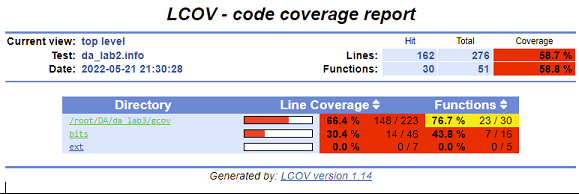
\includegraphics{images/all_proj.png}
    
    Если детальнее посмотреть конктретно покрытия моей программы, то результат будет несколько лучше, однако до 100\% покрытия далеко.\newline
    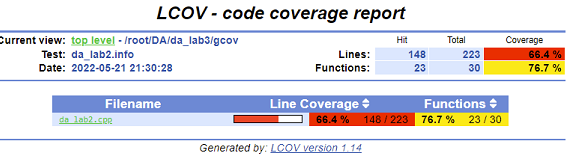
\includegraphics{images/my_prog.png}
    
    Детальный анализ дает понять, что в следствии выбора именно такого теста в программе не используются участки кода с тремя из четырех видов поворота и участки с удалением элементов из деорева.\newline
    
\end{enumerate}

\pagebreak